%%% UNIT 7
{
\setbeamertemplate{headline}{}
\setbeamertemplate{footline}{
  \begin{beamercolorbox}[wd=\paperwidth,ht=2.2ex,dp=1.5ex]{palette quaternary}
  \end{beamercolorbox}
  }
\begin{frame}[noframenumbering]
\frametitle{\DB{\huge{\textbf{$\blacksquare$ Unit 7}}}}
\myPause
 \begin{itemize}
 \item[] \LARGE{\MB{Practice session 3}}
 \item[] \vspace{-1mm}\hspace{5mm}\Large{\MB{Applying PI(D) control and looking at the actions}}
 \item[] \vspace{-1mm}\hspace{5mm}\Large{\MB{The second-order case --- why PID is so general}}
 \item[] \vspace{-1mm}\hspace{5mm}\Large{\MB{Variations over an algorithm}}
 \end{itemize}
\end{frame}
}

\part{}

\section{The PID actions}
\subsection{}

\begin{frame}
\frametitleTC{Foreword}
\framesubtitleTC{}
\myPause
 \begin{itemize}[<+-| alert@+>]
 \item We carry out this treatise in a DT LTI (comments on saturations later on) with sampling time $T_s$.
 \item This said, from the PID quasi-algorithm on slide~\ref{pag:PID-quasi-alg} we get the error-to-action
       transfer functions
       \begin{displaymath}
        \begin{array}{lclcl}
         C_P(z) &:=& \cfrac{u_P(k)}{e(k)} &=& K, \\ \\
         C_I(z) &:=& \cfrac{u_I(k)}{e(k)} &=& \cfrac{KT_s}{T_i} \, \cfrac{z}{z-1}, \\ \\
         C_D(z) &:=& \cfrac{u_D(k)}{e(k)} &=& \cfrac{KT_d(1-\beta)}{T_s} \, \cfrac{z-1}{z-\beta}.
        \end{array}
       \end{displaymath}
 \end{itemize}
\end{frame}

\begin{frame}
\frametitleTC{Foreword}
\framesubtitleTC{}
\myPause
 \begin{itemize}[<+-| alert@+>]
 \item Block diagram of a PID control loop evidencing the three actions
       \begin{center}
        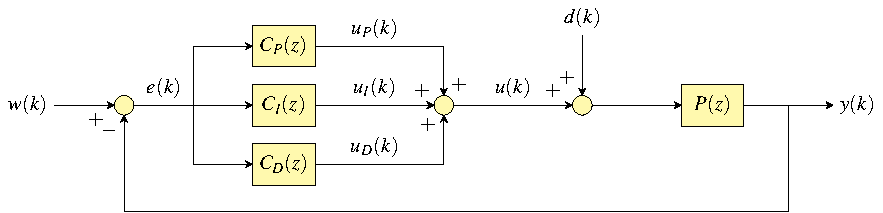
\includegraphics[width=0.85\columnwidth]{./Unit-07/img/PIDloop-actions.pdf}
       \end{center}
 \item \vspace{2mm}NOTE: the disturbance is added to the control signal, i.e., $H(z)=P(z)$;\\
       such a disturbance is called a \TC{load} or a \TC{matched} disturbance.
 \item Load disturbances can arise every time the disturbing and the\\
       control actions are physically homogeneous, which is not infrequent\\
       ---e.g., the control is allocating a resource, and the disturbing entity\\
       is somebody subtracting some amount of the same resource.
 \end{itemize}
\end{frame}

\begin{frame}
\frametitleTC{Computing the three actions}
\framesubtitleTC{}
\myPause
 \begin{itemize}[<+-| alert@+>]
 \item From
       \begin{center}
        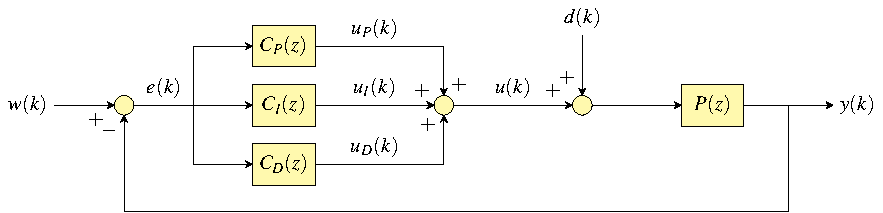
\includegraphics[width=0.70\columnwidth]{./Unit-07/img/PIDloop-actions.pdf}
       \end{center}
       and setting $C(z) = C_P(z)+C_I(z)+C_D(z)$, we readily get
       \begin{displaymath}
        \begin{array}{llcll}
          \cfrac{u_P(k)}{w(k)} &\mkern-12mu =  \cfrac{C_P(z)}{1+P(z)C(z)},       &\quad&
          \cfrac{u_P(k)}{d(k)} &\mkern-12mu = -\cfrac{P(z)C_P(z)}{1+P(z)C(z)}, \\
          \cfrac{u_I(k)}{w(k)} &\mkern-12mu =  \cfrac{C_I(z)}{1+P(z)C(z)},       &\quad&
          \cfrac{u_I(k)}{d(k)} &\mkern-12mu = -\cfrac{P(z)C_I(z)}{1+P(z)C(z)}, \\
          \cfrac{u_D(k)}{w(k)} &\mkern-12mu =  \cfrac{C_D(z)}{1+P(z)C(z)},       &\quad&
          \cfrac{u_D(k)}{d(k)} &\mkern-12mu = -\cfrac{P(z)C_D(z)}{1+P(z)C(z)}.
        \end{array}
       \end{displaymath}
 \end{itemize}
\end{frame}

\begin{frame}
\frametitleTC{Computing the three actions}
\framesubtitleTC{}
\myPause
 \begin{itemize}[<+-| alert@+>]
 \item We now examine the behaviour of the scheme above with a first-order process\\
       with gain $\mu$ and time constant $T$, that recalling slide~\ref{pag:FOsystem-DT}, in transfer function\\
       form reads
       \begin{displaymath}
        P(z) = \frac{\mu\frac{T_s}{T+T_s}z}{z-\frac{T}{T+T_s}}.
       \end{displaymath}
 \item We start out with a PI tuned by cancellation as per the formul{\ae} of slide~\ref{pag:PItuning-lambda},\\
       that is,
       \begin{displaymath}
        K   = \frac{T}{\lambda\mu}, \quad
        T_i = T.
       \end{displaymath}
       where $\lambda$ is the desired closed-loop time constant (1/5 of the desired\\
       settling time).
 \item Then we add a bit of D action, and comment on all of the results.
 \end{itemize}
\end{frame}

\begin{frame}[fragile]
\frametitleTC{Computing the three actions}
\framesubtitleTC{Scilab script (1/3)}
\myPause
 {\scriptsize
 \begin{verbatim}
 clear; clc;                                          // clear workspace & console
 z      = %z;                                         // allow to omit lots of %'s below

 mu     = 1;                                          // process gain  
 T      = 10;                                         // and time constant
 lambda = 4;                                          // desired closed-loop TC
 Beta   = 0.6;                                        // derivative filter
 Ts     = 1;                                          // sampling time
 tfin   = 50;                                         // simulation end time

 K      = T/lambda/mu;                                // PID tuning
 Ti     = T;
 Td     = 0;

 P      = syslin(Ts,z*Ts/(T+Ts)/(z-T/(T+Ts)));        // process and controller
 Cp     = K;                                          // transfer functions:
 Ci     = syslin(Ts,K*Ts/Ti*z/(z-1));                 // a number instead of
 Cd     = syslin(Ts,K*Td*(1-Beta)/Ts*(z-1)/(z-Beta)); // 'd' sets the sampling
 C      = Cp+Ci+Cd;                                   // time for a DT system
 \end{verbatim}
 }
\end{frame}

\begin{frame}[fragile]
\frametitleTC{Computing the three actions}
\framesubtitleTC{Scilab script (2/3)}
\myPause
 {\scriptsize
 \begin{verbatim}
 w2y    = tf2ss(C*P/(1+C*P));           // transfer function from w to y
 d2y    = tf2ss(P/(1+C*P));             // transfer function from d to y
 w2u    = tf2ss(C/(1+C*P));             // transfer function from w to u
 d2u    = tf2ss(-C*P/(1+C*P));          // transfer function from d to u
 w2up   = tf2ss(Cp/(1+C*P));            // transfer function from w to up
 w2ui   = tf2ss(Ci/(1+C*P));            // transfer function from w to ui
 w2ud   = tf2ss(Cd/(1+C*P));            // transfer function from w to ud
 d2up   = tf2ss(-P*Cp/(1+C*P));         // transfer function from d to up
 d2ui   = tf2ss(-P*Ci/(1+C*P));         // transfer function from d to ui
 d2ud   = tf2ss(-P*Cd/(1+C*P));         // transfer function from d to ud

 t      = 0:Ts:tfin;                    // time vector
 wd     = ones(t);                      // step with one zero sample 
 wd(1)  = 0;                            // at the beginning
 yw     = dsimul(w2y,wd)';              // y in response to a w step
 yd     = dsimul(d2y,wd)';              // y in response to a d step
 uw     = dsimul(w2u,wd)';              // u in response to a w step
 ud     = dsimul(d2u,wd)';              // u in response to a d step
 upidw  = dsimul([w2up;w2ui;w2ud],wd)'; // u{p,i,d} in response to a w step
 upidd  = dsimul([d2up;d2ui;d2ud],wd)'; // u{p,i,d} in response to a d step
 \end{verbatim}
 }
\end{frame}

\begin{frame}[fragile]
\frametitleTC{Computing the three actions}
\framesubtitleTC{Scilab script (3/3)}
\myPause
 {\scriptsize
 \begin{verbatim}
 hf=scf(0); clf; hf.figure_size = [1200,700];                    // plot stuff: see the Scilab
 subplot(321); title('Responses to a w unit step'); ylabel('y'); // documentation for technical
   plot(0,0,'k');                                                // details here inessential
   plot(t',ones(t'),'k:');
   plot(t',yw,'b','linewidth',4);
 subplot(322); title('Responses to a d unit step'); 
   plot(t',zeros(t'),'k:');
   plot(t',yd,'b','linewidth',4);
 subplot(323); xlabel('time'); ylabel('u,up,ui,ud (g,b,r,m)');
   plot(0,0,'k');
   plot(t',uw,'g','linewidth',4);
   plot(t',upidw(:,1),'b','linewidth',2);
   plot(t',upidw(:,2),'r','linewidth',2);
   plot(t',upidw(:,3),'m','linewidth',2);
 subplot(324); xlabel('time');
   plot(0,0,'k');
   plot(t',ud,'g','linewidth',4);
   plot(t',upidd(:,1),'b','linewidth',2);
   plot(t',upidd(:,2),'r','linewidth',2);
   plot(t',upidd(:,3),'m','linewidth',2);
 \end{verbatim}
 }
\end{frame}

\begin{frame}
\frametitleTC{Observing the three actions}
\framesubtitleTC{Scilab script -- example of the output}
\myPause
 \begin{center}
  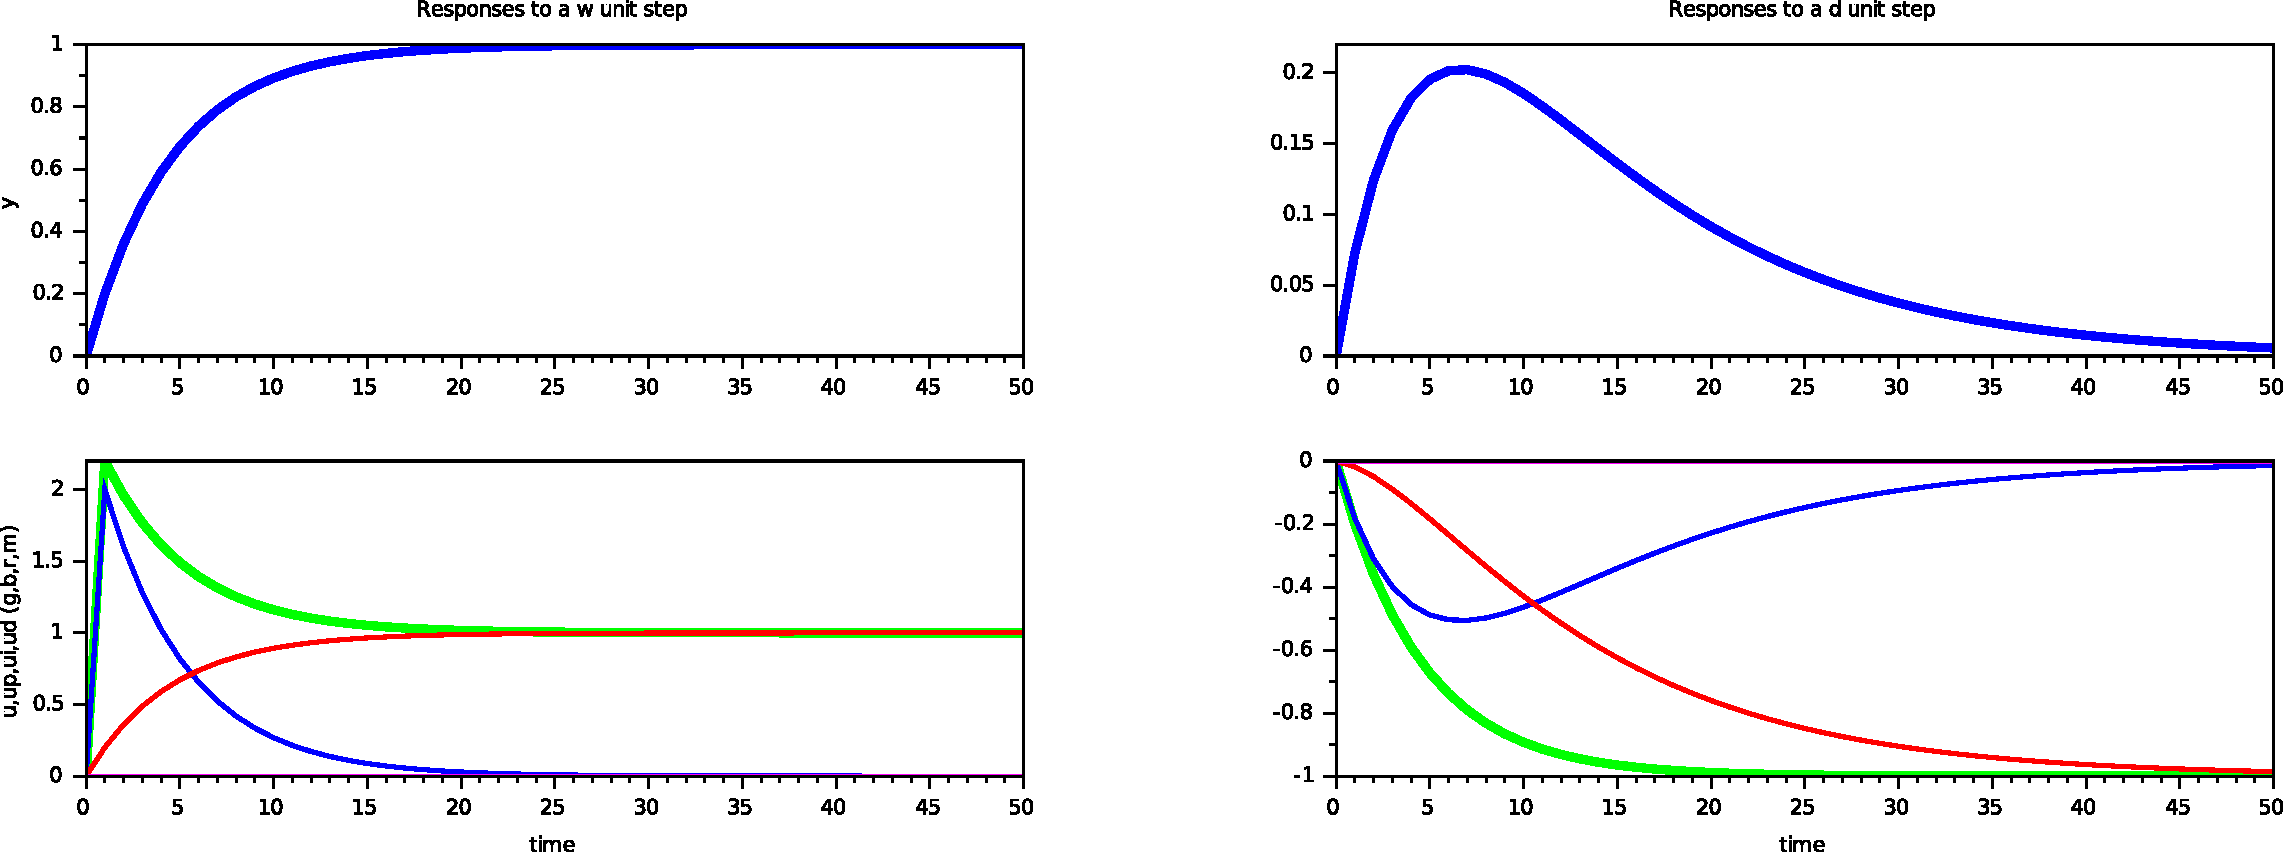
\includegraphics[width=0.75\columnwidth]{./Unit-07/img/PIDactions-scilab-01.pdf}
 \end{center}
 \begin{itemize}[<+-| alert@+>]
 \item Top row: responses of $y$ to a unit step on $w$ (left) and on $d$ (right).
 \item Bottom row: breakdown of $u$ (green) into $u_P$ (blue), $u_I$ (red),\\
       and $u_D$ (magenta).
 \item Note that at steady state $u$ is made only of integral action.
 \item Let us now play around with PID parameters, also not following the\\
       tuning rule exactly, and see what happens.
 \end{itemize}
\end{frame}

\begin{frame}[fragile]
\frametitleTC{Observing the three actions}
\framesubtitleTC{Playing around with PID parameters -- a few suggestions (1/3)}
\myPause
 \begin{itemize}[<+-| alert@+>]
 \item Add some D action:
       {\scriptsize
       \begin{verbatim}
       K   = T/lambda/mu;
       Ti  = T;
       Td  = 0.2*Ti;
       \end{verbatim}
       }
 \item \vspace{-3mm}Speeds up initial transient, hardly any effect on settling time, just a \emph{very} small\\
       overshoot:
       \begin{center}
        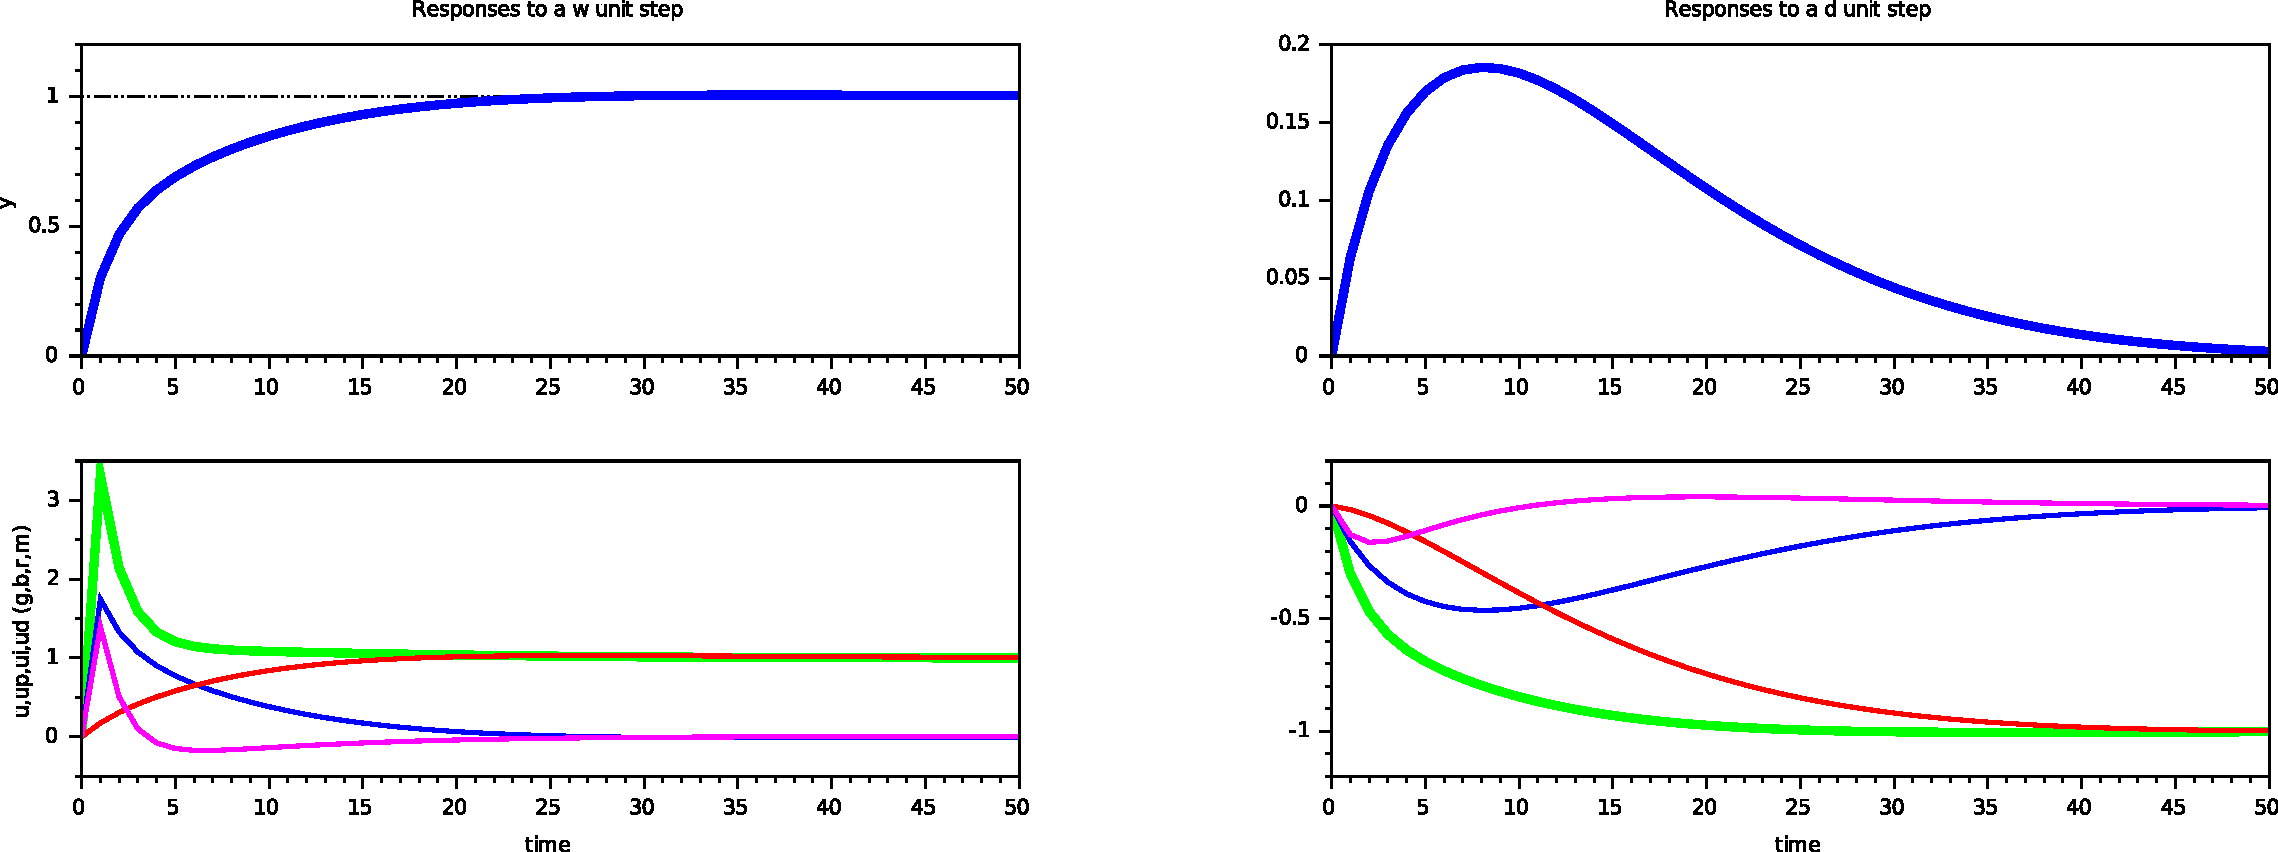
\includegraphics[width=0.60\columnwidth]{./Unit-07/img/PIDactions-scilab-02.pdf}
       \end{center}
 \item Note that clearly the D action vanishes as well toward steady state \\
       (and faster than P). 
 \end{itemize}
\end{frame}

\begin{frame}[fragile]
\frametitleTC{Observing the three actions}
\framesubtitleTC{Playing around with PID parameters -- a few suggestions (2/3)}
\myPause
 \begin{itemize}[<+-| alert@+>]
 \item Back to PI, but halve the integral time:
       {\scriptsize
       \begin{verbatim}
       K   = T/lambda/mu;
       Ti  = 0.5*T;
       Td  = 0;
       \end{verbatim}
       }
 \item \vspace{-3mm}Disturbance response improved at the cost of a slight oscillation\\
       ---i.e., some stability reduction:
       \begin{center}
        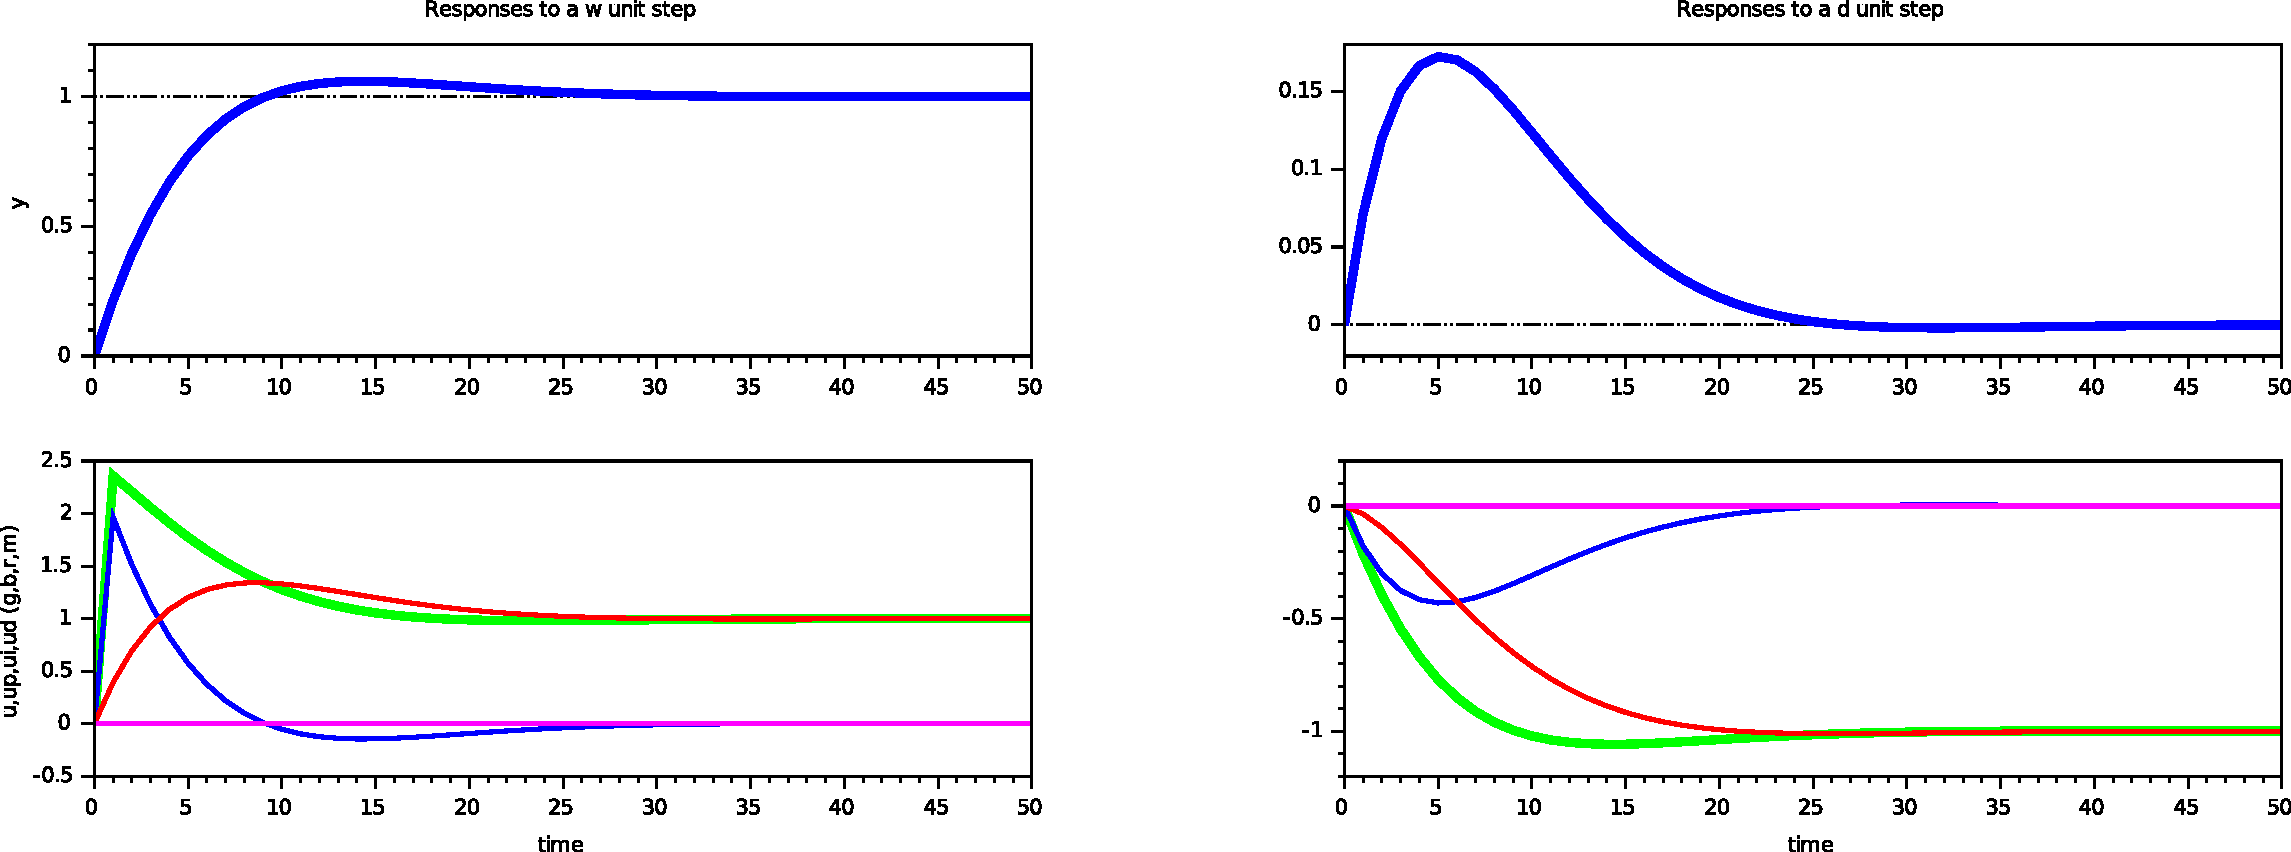
\includegraphics[width=0.60\columnwidth]{./Unit-07/img/PIDactions-scilab-03.pdf}
       \end{center}
 \item Try adjusting $K$ to eliminate the oscillation in the set point response.\\
       Do you succeed? Or just alter the oscillation period?
 \end{itemize}
\end{frame}

\begin{frame}[fragile]
\frametitleTC{Observing the three actions}
\framesubtitleTC{Playing around with PID parameters -- a few suggestions (3/3)}
\myPause
 \begin{itemize}[<+-| alert@+>]
 \item PID again, but with a definitely excessive integral time:
       {\scriptsize
       \begin{verbatim}
       K   = T/lambda/mu;
       Ti  = 4*T;
       Td  = 0.2*Ti;
       \end{verbatim}
       }
 \item \vspace{-3mm}When P and D vanish, I is still far from playing its full role:
       \begin{center}
        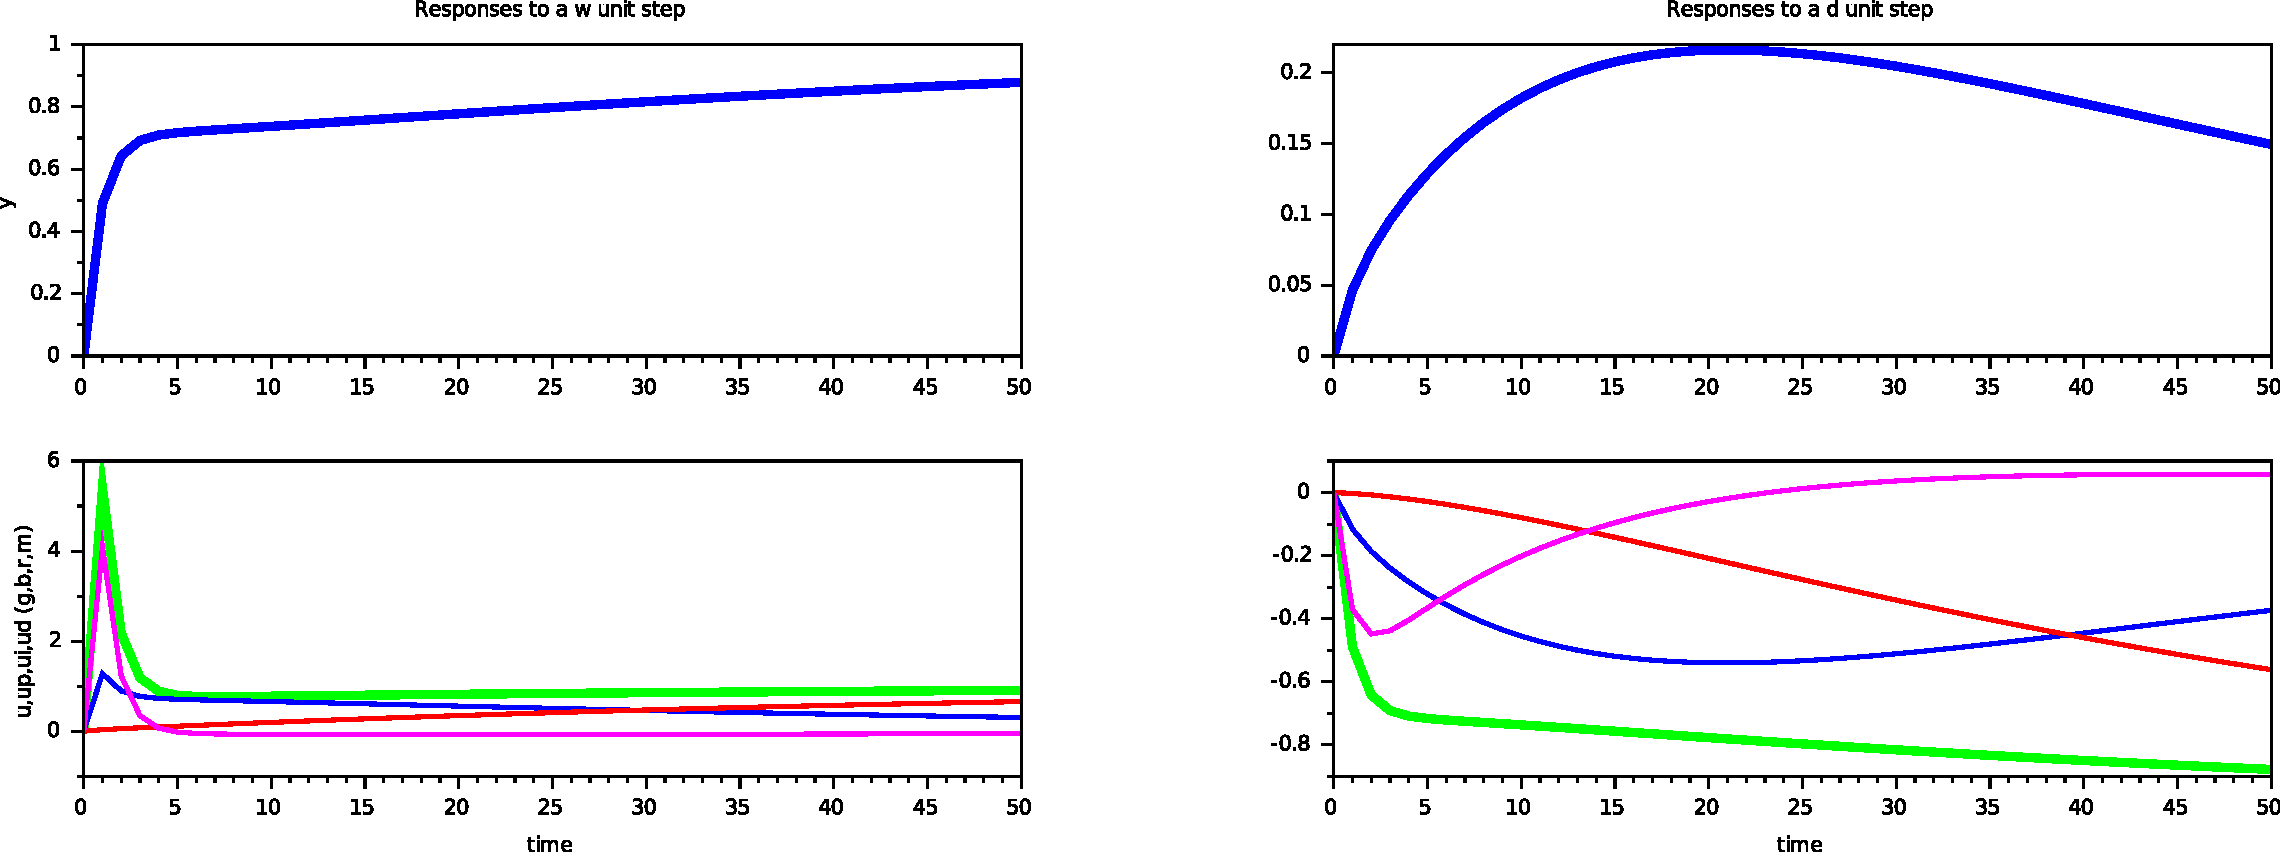
\includegraphics[width=0.60\columnwidth]{./Unit-07/img/PIDactions-scilab-04.pdf}
       \end{center}
 \item Try removing the D action. What effects do you observe on the set\\ 
       point and the disturbance response? Do these correspond to your\\
       expectations?
 \end{itemize}
\end{frame}

\begin{frame}[fragile]
\frametitleTC{The P, I, and D actions}
\framesubtitleTC{Suggestions for further activities}
\myPause
 \begin{itemize}[<+-| alert@+>]
 \item Take the Scilab script above and add some noise on the feedback path---i.e., the \TC{measurement}
       of $y$ fed back to $C$ is corrupted by noise. Hint: Scilab has a \texttt{rand()} and a \texttt{randn()}
       function for uniformly and normally distributed random numbers.
 \item Always remember:
       \begin{itemize}[<+-| alert@+>]
       \item we would like to control physical quantities,
       \item but we can only control measurements.
       \end{itemize}
 \item \vfill Experiment with different numbers, observe, and comment.
 \end{itemize}
\end{frame}

\begin{frame}[fragile]
\frametitleTC{The P, I, and D actions}
\framesubtitleTC{Takeaways}
\myPause
 \begin{itemize}[<+-| alert@+>]
 \item Looking at a response and diagnosing: too much P action, too few I,...
 \item A keyword for the curious here is ``tuning maps''.
 \item \vspace{2mm} Use your \TC{systems theory} knowledge to confirm or debunk some common beliefs:
       \begin{itemize}[<+-| alert@+>]
       \item adding D always makes a system faster --- sure, given one of the tests above?
       \item too much D destabilises --- hmmm, or maybe just amplifies noise?
       \item increasing $K$ does not reject disturbances faster, for that you need\\
             to reduce $T_i$ --- i.e., not just tune by cancellation,
       \item ...and so forth.
       \end{itemize}
 \item If interested go through the many PID-related web sites, read, test\\
       (you have \TC{methods} \& tools) and subject the material you found\\
       to a system-theoretically educated analysis.
 \item This is what we meant right from the outset for ``using (PID)\\
       control consciously''. 
 \end{itemize}
\end{frame}

%Myths debunked
% D makes faster...

%Lessons learnt:
% diagnose, tuning maps


\section{Why PID is so generally applicable}
\subsection{}

\begin{frame}
\frametitleTC{The second-order process case}
\framesubtitleTC{aka ``one size fits many''}
\myPause
 \begin{itemize}[<+-| alert@+>]
 \item We consider an asymptotically  process with two poles and one zero at most, i.e.,
       \begin{displaymath}
        P(z) = \mu \frac{z-z_1}{(z-p_1)(z-p_2)}, \qquad |p_{1,2}|<1.
       \end{displaymath}
 \item We want to show that this gives rise to the four possible cases
       \begin{displaymath}
        \begin{array}{rcll}
         P_1(z) &=& \frac{\mu}{z-p_1},                                               \\
         P_2(z) &=& \frac{\mu}{(z-p_1)(z-p_2)},                                      \\
         P_3(z) &=& \frac{\mu(z-z_1)}{(z-p_1)(z-p_2)}, & |z_1|<1,                    \\
         P_4(z) &=& \frac{\mu(z-z_1)}{(z-p_1)(z-p_2)}, & |z_1|>1 \text{ or } z_1=-1, \\
        \end{array}
       \end{displaymath}
       and that each of these is very naturally paired to a PI(D) controller.
 \item But: why not a case with one pole and one zero? Why not $z_1=1$?
 \item We need another short \emph{intermezzo}...
 \end{itemize}
\end{frame}

\begin{frame}
\frametitleTC{Why not $z_1=1$}
\framesubtitleTC{}
\myPause
 \begin{itemize}[<+-| alert@+>]
 \item We start from the simple. If $z_1=1$ the process output $y$ tends asymptotically to zero
       for any constant input $u$, as it comes to depend on $u(k)-u(k-1)$.
 \item This means that to keep $y$ at a certain constant reference value, $u$ should indefinitely
       increase at a corresponding constant \TC{rate}, up to infinity---or overflow.
       Apparently, such a process cannot be managed (control people use to say ``you cannot prescribe
       the steady state'').
 \item If conversely $z_1=-1$ one can prescribe the steady state, but not cancel the zero with a
       pole of $C$, or the cancellation would be critical, as we already know.
 \item We thus consider $z_1=-1$ and $|z_1|>1$ the same case, and we know\\
       what the outcome will be.
 \item More interesting is to discuss why we assume $P$ to be always strictly\\
       proper (more poles than zeroes). 
 \end{itemize}
\end{frame}

\begin{frame}
\frametitleTC{A controller's execution timeline}
\framesubtitleTC{Some considerations}
\myPause
 \begin{itemize}[<+-| alert@+>]
 \item Let us first point a further peculiarity of control in computers.
       \begin{itemize}[<+-| alert@+>]
       \item When the controlled object is outside the computer, it always evolves in \TC{physical}
             parallel with the controller's execution; when it is inside, that parallel might be physical
             or just emulated, if the two entities share a CPU. Said otherwise, \TC{running the controller
             can halt the process}.
       \item More in general, in non-computer applications, running controllers adds value to the process
             by improving its operation. In computers, on the contrary, time to compute the control signals
             is \TC{anyway stolen} from that devoted to applications. And since value ultimately comes from
             running applications, time for running controllers must be almost negligible.
       \end{itemize}
 \item For the sake of completeness, the second statement may not hold\\
       if the control payback is really huge, or if controllers have dedicated\\
       hardware to run; we leave discussing such cases to advanced\\
       activities, however.
 \end{itemize}
\end{frame}

\begin{frame}
\frametitleTC{A controller's execution timeline}
\framesubtitleTC{Some considerations}
\myPause
 \begin{itemize}[<+-| alert@+>]
 \item In general -- i.e., considering also cases we do not address in our activity -- one can distinguish
       three cases (thinking for simplicity of a sampled signals context):
       \begin{itemize}[<+-| alert@+>]
       \item the time $\tau(k)$ to compute the generic $u(k)$ is negligible wrt the sampling period $T_s$;
       \item $\tau(k)$ is not negligible wrt $T_s$ but it is -- almost -- invariant (no branches, no operations
             with operand-dependent duration, no or negligible cache effects, and so on---or countermeasures taken
             in the code for such issues);
       \item $\tau(k)$ is not negligible wrt $T_s$ and can vary significantly over the control steps.
       \end{itemize}
 \item We do not have the time to investigate the matter (but those who want to deal\\
       safely with high-performance real-time control \TC{should} study it very\\
       carefully in control technology courses).
 \item In fact a PI(D) algorithm can be made very lightweight (down to a\\
       few tens of clock cycles, to give a figure) so that we are practically\\
       always in the first case.
 \end{itemize}
\end{frame}

\begin{frame}
\frametitleTC{A controller's execution timeline}
\framesubtitleTC{Some considerations}
\myPause
 \begin{itemize}[<+-| alert@+>]
 \item The timeline is therefore as follows:
       \begin{center}
        \vspace{1mm}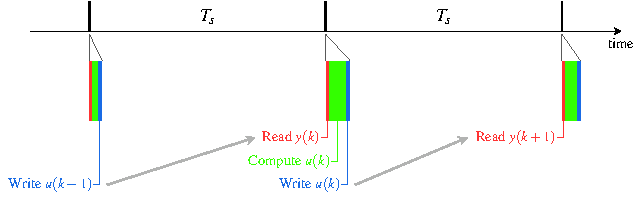
\includegraphics[width=0.70\columnwidth]{./Unit-07/img/CtrlTimeline.pdf}
       \end{center}
 \item As can be seen, the effect of $u(k)$ can be seen only at step $k+1$,\\
       hence the process is correctly viewed as a strictly proper model.
 \item Incidentally, being in the first case is essential to make the P action\\
       possible.
 \item ...end of the \emph{intermezzo}.
 \end{itemize}
\end{frame}

\begin{frame}
\frametitleTC{Back to the second-order process}
\framesubtitleTC{for a reasoned recap and a systematisation}
\myPause
 \begin{itemize}[<+-| alert@+>]
 \item Exercise: take the four cases
       \begin{displaymath}
        \begin{array}{rcll}
         P_1(z) &=& \frac{\mu}{z-p_1},                                               \\
         P_2(z) &=& \frac{\mu}{(z-p_1)(z-p_2)},                                      \\
         P_3(z) &=& \frac{\mu(z-z_1)}{(z-p_1)(z-p_2)}, & |z_1|<1,                    \\
         P_4(z) &=& \frac{\mu(z-z_1)}{(z-p_1)(z-p_2)}, & |z_1|>1 \text{ or } z_1=-1. \\
        \end{array}
       \end{displaymath}
 \item For each of them select a controller structure, devise a way to provide\\
       a response speed specification, and formalise a tuning procedure;\\
       then build a Modelica LTI scheme to simulate the so obtained\\
       loops, design and carry out experiments, and comment.
 \end{itemize}
\end{frame}


\section{Variations over an algorithm}
\subsection{}

\begin{frame}
\frametitleTC{Foreword}
\framesubtitleTC{}
\myPause
 \begin{itemize}[<+-| alert@+>]
 \item Now we know enough for our purposes about the PID control law.
 \item We also know that to turn the LTI law into an algorithm, there are some nonlinear additions
       to care about (e.g., antiwindup).
 \item Such additions are not just ``implementation choices''; they do not fit into the LTI
       context, but nonetheless \TC{need addressing systematically}.
 \item Otherwise the (wrong) conclusion is easily reached that ``the theory is neat but too
       simplistic to be useful in the real world''...
 \item ...and controls soon become an inextricable and unmaintainable\\
       \emph{spaghetti} code, where -- inexplicably from the control scientist's\\
       viewpoint --  problems are tackled by adding further complexity\\
       (apologies for not resisting the temptation to this remark).
 \end{itemize}
\end{frame}

\begin{frame}
\frametitleTC{Foreword}
\framesubtitleTC{}
\myPause
 \begin{itemize}[<+-| alert@+>]
 \item Anticipating a bit, we want to reach the following conclusions:
       \begin{itemize}[<+-| alert@+>]
       \item you tune and assess a PID, or more in general a control scheme,\\
             in the LTI context,
       \item and then you take care of ``nonlinear additions'' in such a way\\
             to not contradict/disrupt your LTI findings;
       \item but to make this possible, a PID block must contain something\\
             more than the LTI law (and this we are going to study a bit).
       \end{itemize}
 \item Given the available space, here we address ``algorithm variations'' -- i.e.,\\
       the ``something more'' above -- as for three aspects only:
       \begin{itemize}[<+-| alert@+>]
       \item positional versus incremental form,
       \item how antiwindup is realised,
       \item and (a few examples of) what can be added to ease interconnecting\\
             a PID with other controllers in the same overall system.
       \end{itemize}
 \item \vfill Once again, much more in advanced control (technology) courses.
 \end{itemize}
\end{frame}

\begin{frame}
\frametitleTC{Positional vs. incremental realisation}
\framesubtitleTC{Definition}
\myPause
 \begin{itemize}[<+-| alert@+>]
 \item For simplicity in this treatise we refer to a PI, conceptually nothing changes\\
       if D is added.
 \item \vspace{2mm} \TC{Positional} realisation:\\
       $e(k)$ is used to compute $u(k)$.
 \item \vspace{2mm} \TC{Incremental} realisation:\\
       first the variation of $u(k)$ wrt its previous value is computed,\\
       and then this variation is added to the previous value of $u$ to get\\
       the current one.
 \end{itemize}
\end{frame}

\begin{frame}
\frametitleTC{Positional vs. incremental realisation}
\framesubtitleTC{The variation operator}
\myPause
 \begin{itemize}[<+-| alert@+>]
 \item We define the \TC{variation operator} $\Delta$ with reference to the one-step advance\\
       one $z$, as
       \begin{displaymath}
        \Delta := 1-z^{-1}.
       \end{displaymath}
 \item As a consequence, since in the time domain the variation of a signal $v(k)$
       is naturally defined as
       \begin{displaymath}
        \Delta v(k) = v(k)-v(k-1),
       \end{displaymath}
       we can give the formal multiplication by $\Delta$ an operatorial sense,\\
       exactly as we in fact already did for the formal multiplication by $z$. 
 \end{itemize}
\end{frame}


\begin{frame}
\frametitleTC{Positional vs. incremental realisation}
\framesubtitleTC{An incremental PI}
\myPause
 \begin{itemize}[<+-| alert@+>]
 \item The positional PI law, as we already know, is
       \begin{displaymath}
        \begin{array}{rcl}
         u_P(k) &=& K e(k) \\
         u_I(k) &=& u_I(k-1) + \cfrac{KT_s}{T_i} e(k)
        \end{array}
       \end{displaymath}
 \item hence the incremental one readily stems from the definition of $\Delta$, as
       \begin{displaymath}
        \begin{array}{rcl}
         \Delta u_P(k) &=& K \Delta e(k) \\
         \Delta u_I(k) &=& \cfrac{KT_s}{T_i} e(k)
        \end{array}
       \end{displaymath}
       and obviously the control variation $\Delta u(k)$ is just $\Delta u_P(k)+\Delta u_I(k)$.
 \end{itemize}
\end{frame}

\begin{frame}
\frametitleTC{Incremental realisation}
\framesubtitleTC{Pros and cons}
\myPause
 \begin{itemize}[<+-| alert@+>]
 \item Pros:
       \begin{itemize}[<+-| alert@+>]
       \item can use all the available precision for the control \TC{variation},\\
             i.e., just one many-bits register is needed to store $u(k)$, which may be\\
             relevant e.g. when constrained to integer-numbers arithmetic like in the\\
             Linux kernel;
       \item easy to realise antiwindup and tracking (see algorithm later on);
       \end{itemize}
 \item Cons:
       \begin{itemize}[<+-| alert@+>]
       \item for the same reason above, unnatural to realise antiwindup if not in the\\
             ``natural way'' mentioned above (no pun intended);
       \item in the absence of I action \TC{MUST} be in automatic mode when the\\
             set point is varied, otherwise that variation is lost forever.
       \end{itemize}
 \end{itemize}
\end{frame}

\begin{frame}[fragile]
\frametitleTC{Positional vs. incremental realisation}
\framesubtitleTC{PI algorithm example -- positional version from slide~\ref{pag:PI-complete-alg}}
\myPause
 \begin{itemize}[<+-| alert@+>]
 \item[]{\scriptsize
   \begin{verbatim}
// POSITIONAL                                // INCREMENTAL
e      = w-y;                                e       = w-y; 
up     = K*e;                                Delta_e = e-e_old;              
if not TS then                               if not TS then    
   ui  = ui_old+K*Ts/Ti*e;                      Delta_up = K*Delta_e;
   u   = up+ui;                                 Delta_ui = K*Ts/Ti*e;
                                                u        = u_old+Delta_up+Delta_ui;
else                                         else                 
   u   = TR;                                    u        = TR;
end if;                                      end if
u      = max(umin,min(umax,u));              u     = max(umin,min(umax,u));
ui_old = u-up;                               u_old = u;
                                             e_old = e;
   \end{verbatim}
   }
 \item Exercise: try this in Modelica.
 \end{itemize}
\end{frame}

\begin{frame}[fragile]
\frametitleTC{Antiwindup methods}
\framesubtitleTC{}
\myPause
 \begin{itemize}[<+-| alert@+>]
 \item Till now we have been realising antiwindup
       \begin{itemize}[<+-| alert@+>]
       \item either by \TC{integral recomputation} in the positional form, i.e.,\\
             \verb£ u      = max(umin,min(umax,u));£\\
             \verb£ ui_old = u-up;                 £
       \item or by just computing $\Delta u$ (incremental form) and clamping the state of\\
             the \TC{output integrator} that sums the subsequent variations into $u$. 
       \end{itemize}
  \item \vspace{2mm} These methods came naturally, but there are alternatives, and these\\
        may impact the control loop behaviour in the face of large input\\
        (set point or disturbance) swings.
  \item We just see one example, namely antiwindup by \TC{internal positive\\
        feedback}. % NOTE in the future may add actuation error feedback, possibly with actuator model
  \end{itemize}
\end{frame}

\begin{frame}
\frametitleTC{Antiwindup methods}
\framesubtitleTC{PI with antiwindup by internal positive feedback}
\myPause
 \begin{itemize}[<+-| alert@+>]
  \item Block diagram
        \begin{center}
         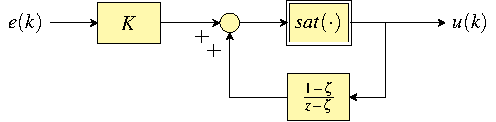
\includegraphics[width=0.60\columnwidth]{./Unit-07/img/PI-AW-intFB.pdf}
        \end{center}
        where for compactness we use the pure DT parametrisation $(K,\zeta)$.
  \item The saturation function is defined as
        \begin{displaymath}
         sat(x) = \begin{cases}
                   \; x_{min} & \quad x < x_{min} \\
                   \; x       & \quad x_{min} \leq x \leq x_{max} \\
                   \; x_{max} & \quad x > x_{max}
                  \end{cases}
        \end{displaymath}
  \end{itemize}
\end{frame}

\begin{frame}
\frametitleTC{Antiwindup by internal positive feedback}
\framesubtitleTC{Operation}
\myPause
 \begin{center}
  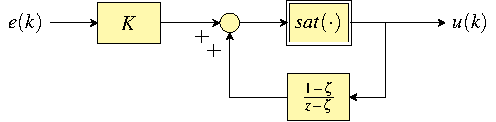
\includegraphics[width=0.45\columnwidth]{./Unit-07/img/PI-AW-intFB.pdf}
 \end{center}
 \myPause
 \begin{itemize}[<+-| alert@+>]
  \item In the absence of saturation the $sat(\cdot)$ block has output=input, hence in transfer function form
        (mind the \red{positive} feedback) we get
        \begin{displaymath}
         \frac{u(k)}{e(k)} = K \frac{1}{1\mathbf{\red{-}}\frac{1-\zeta}{z-\zeta}}
                           = K \frac{z-\zeta}{z-\cancel{\zeta}-1+\cancel{\zeta}}
                           = K \frac{z-\zeta}{z-1}
        \end{displaymath}
        which is a PI as desired.
  \item In the presence of saturation the loop inside the PI opens and the\\
        integrator (see above) ceases to exist  $\Rightarrow$ no windup.
  \end{itemize}
\end{frame}

\begin{frame}
\frametitleTC{Antiwindup PI}
\framesubtitleTC{Modelica (block diagram) representation -- positional realisation}
\myPause
 \begin{center}
  %rsvg-convert -f pdf -o PI_nnn.pdf PI_nnn.svg
  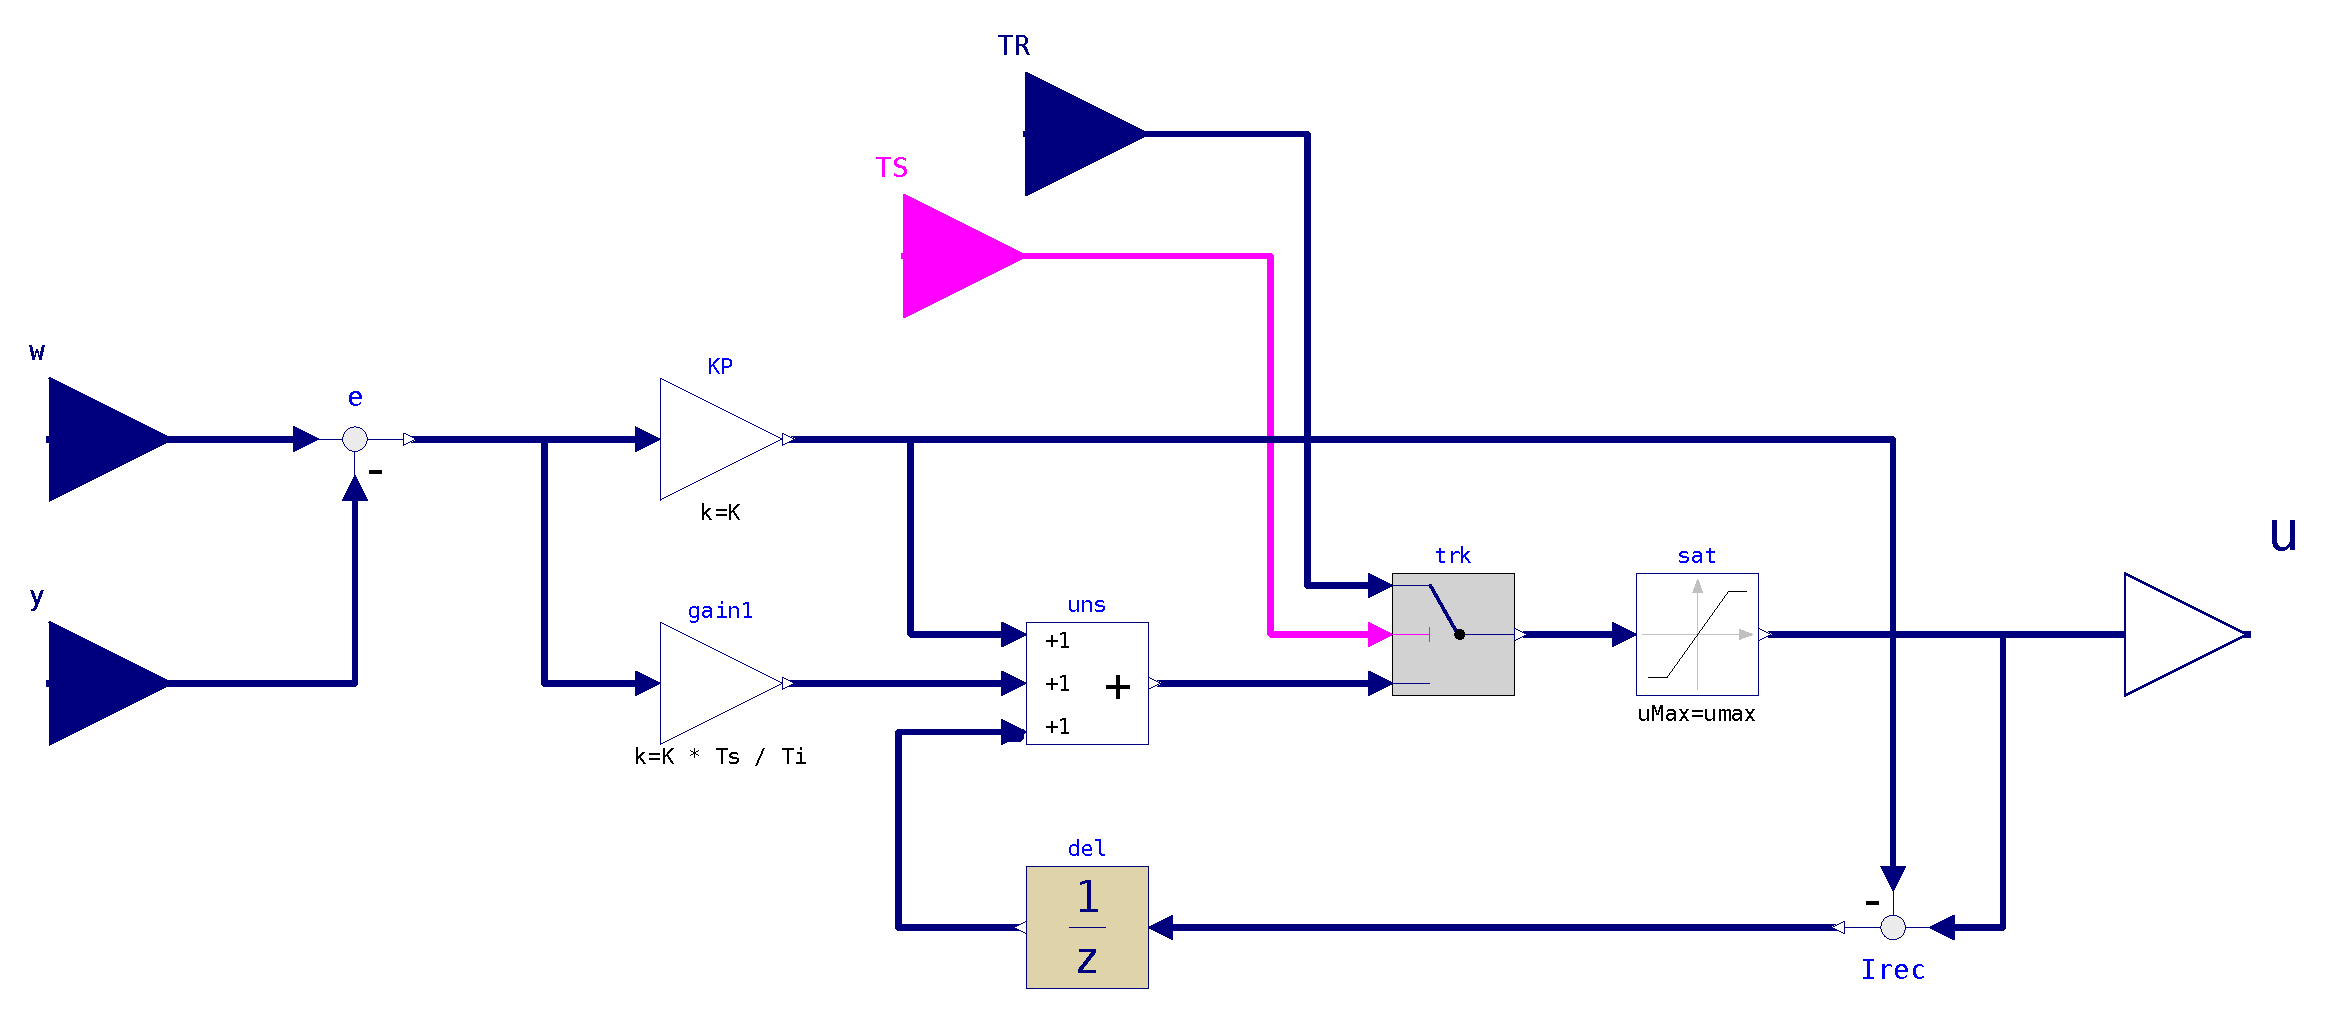
\includegraphics[width=0.80\columnwidth]{./Unit-07/img/PI_POS.pdf}\\
 \end{center}
\end{frame}

\begin{frame}
\frametitleTC{Antiwindup PI}
\framesubtitleTC{Modelica (block diagram) representation -- incremental realisation}
\myPause
 \begin{center}
  %rsvg-convert -f pdf -o PI_nnn.pdf PI_nnn.svg
  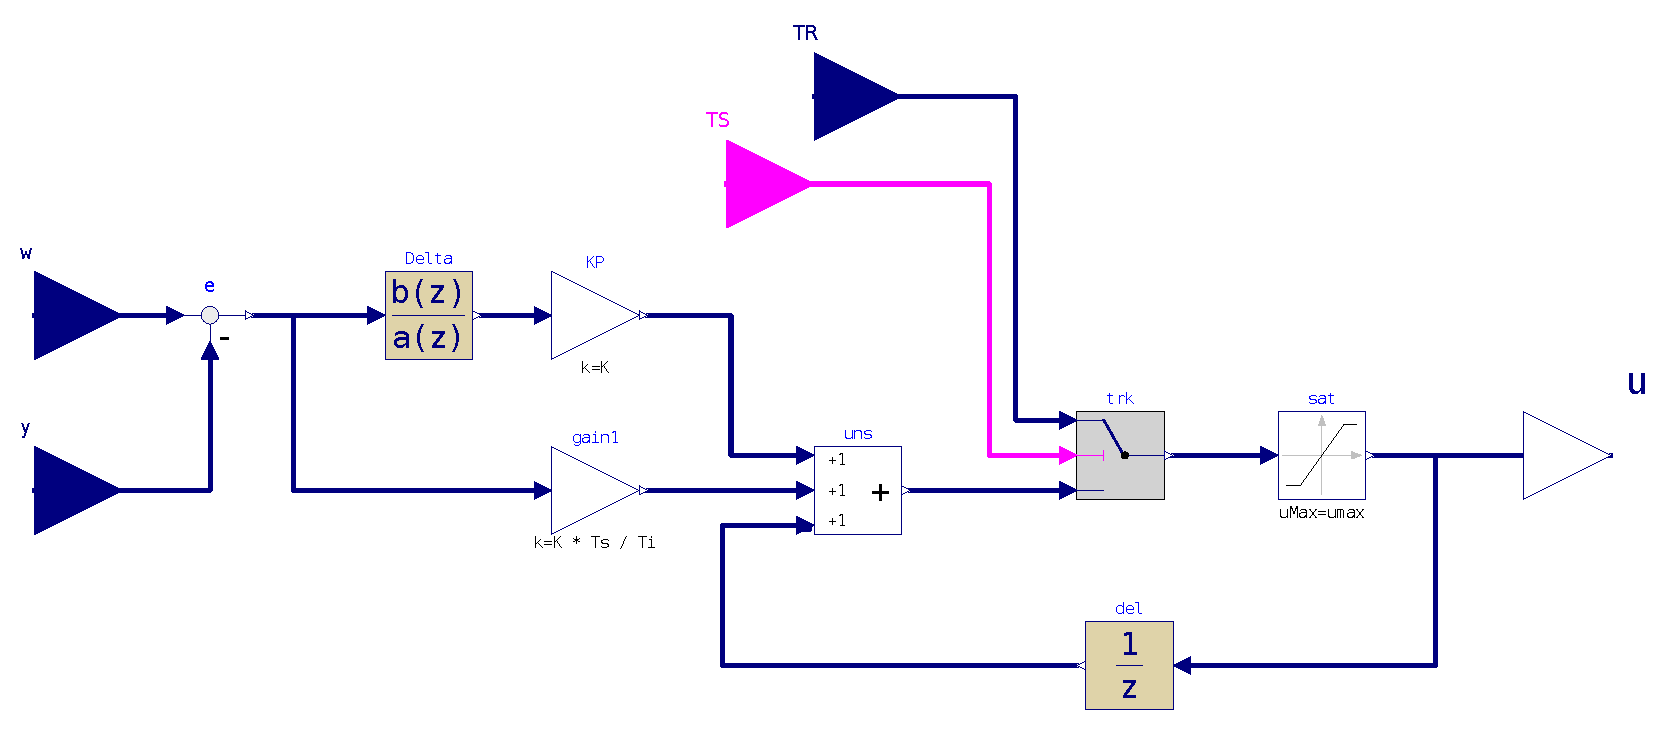
\includegraphics[width=0.80\columnwidth]{./Unit-07/img/PI_INC.pdf}\\
 \end{center}
\end{frame}

\begin{frame}
\frametitleTC{Antiwindup PI}
\framesubtitleTC{Modelica (block diagram) representation -- internal feedback realisation}
\myPause
 \begin{center}
  %rsvg-convert -f pdf -o PI_nnn.pdf PI_nnn.svg
  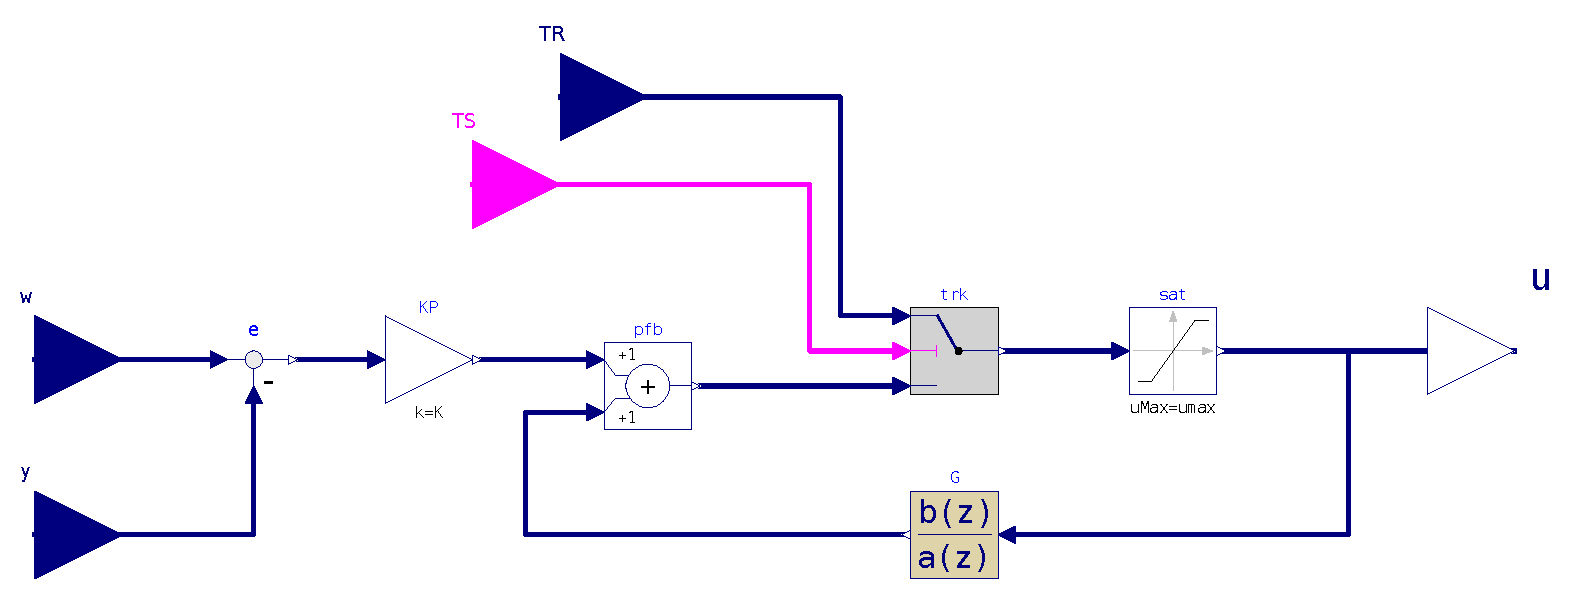
\includegraphics[width=0.80\columnwidth]{./Unit-07/img/PI_IFB.pdf}\\
 \end{center}
\end{frame}

\begin{frame}
\frametitleTC{Antiwindup PI}
\framesubtitleTC{Results and comparison -- set point step large enough to provoke control saturation}
\myPause
 \begin{columns}
  \column[T]{0.70\textwidth}
   \begin{tabular}{ll}
    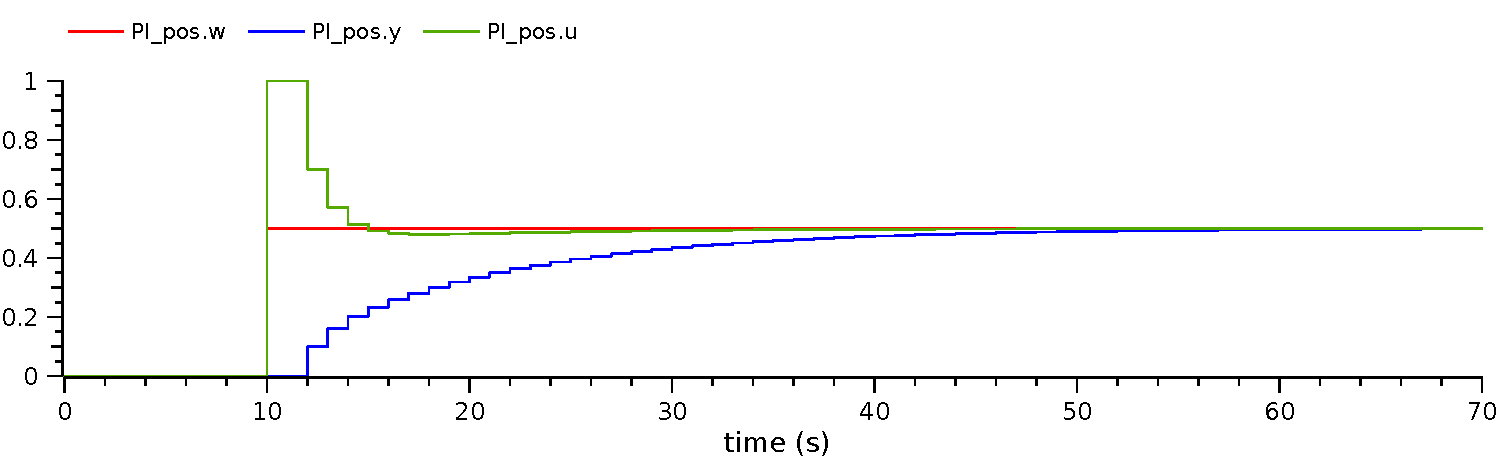
\includegraphics[width=0.70\columnwidth]{./Unit-07/img/PI_POS-wyu.pdf} & Positional
   \end{tabular}
   \begin{tabular}{ll}
    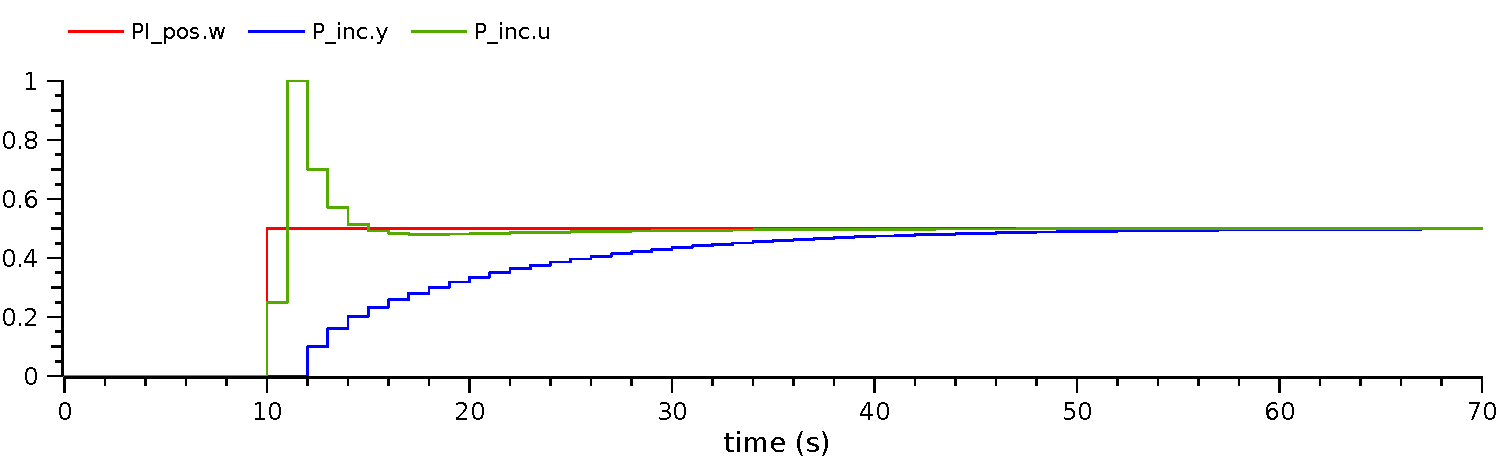
\includegraphics[width=0.70\columnwidth]{./Unit-07/img/PI_INC-wyu.pdf} & Incremental\\
   \end{tabular}
   \begin{tabular}{ll}
    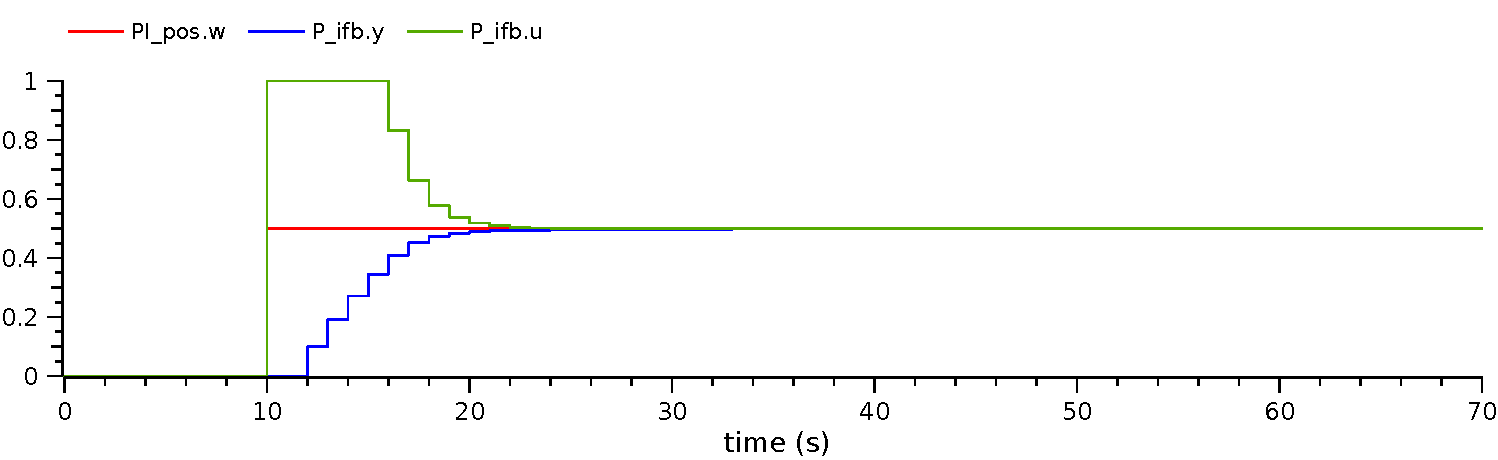
\includegraphics[width=0.70\columnwidth]{./Unit-07/img/PI_IFB-wyu.pdf} & Int. feedback\\
   \end{tabular}
  \column[T]{0.30\textwidth}
   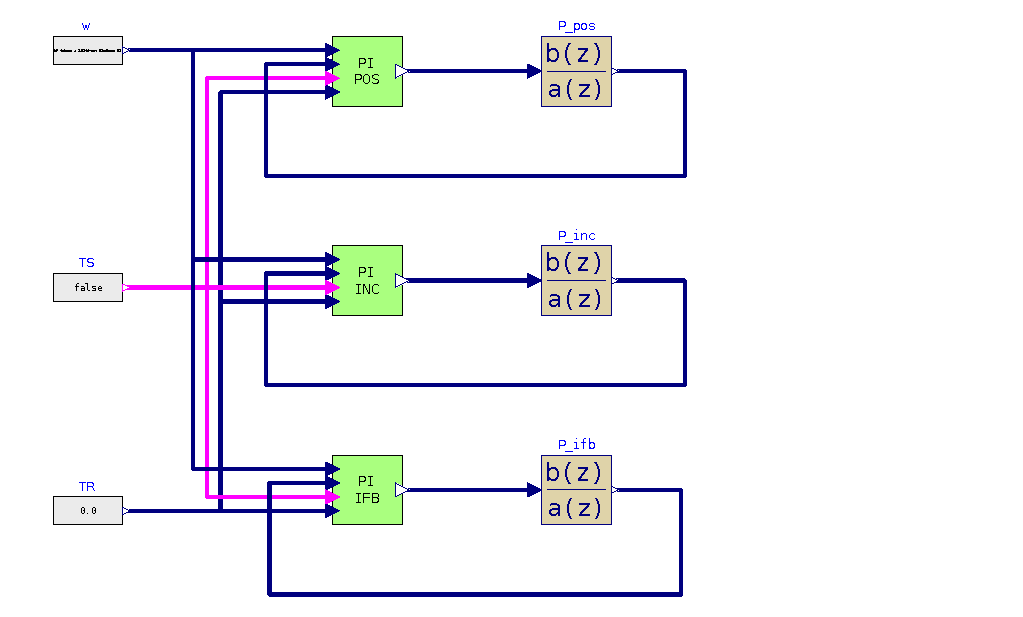
\includegraphics[width=1.20\columnwidth]{./Unit-07/img/AWtypes_ex01.pdf}\\
 \end{columns}
\end{frame}


\section{Conclusions}
\subsection{}

\begin{frame}
\frametitleTC{Conclusions}
\framesubtitleTC{Recap and lessons learnt}
\myPause
 \begin{itemize}[<+-| alert@+>]
 \item Observing and interpreting the P, I and D actions.
 \item Relating the wide applicability of PID control to the wide representativeness of second order models.
 \item Retaining that
       \begin{itemize}[<+-| alert@+>]
       \item \TC{the structure of a control law is dictated by that of the process dynamics
             and not only by the desired closed-loop behaviour},
       \item and \TC{if the structure is properly chosen, setting parameters follows quite\\
             naturally} (while otherwise it can be trial-and-error to eternity),
       \item hence in the absence of some Systems and Control theory knowledge,\\
             there is simply no way out (if not in trivial cases).      
       \end{itemize}
 \end{itemize}
\end{frame}

\begin{frame}
\frametitleTC{Conclusions}
\framesubtitleTC{Recap and lessons learnt}
\myPause
 \begin{itemize}[<+-| alert@+>]
 \item The basics about the timeline of a control loop and the related problems.
 \item Accounting properly for (some) algorithm-related facts not shown in the LTI context, namely
       \begin{itemize}[<+-| alert@+>]
       \item positional vs. incremental form,
       \item and antiwindup type.
       \end{itemize}
 \item Understanding the potential effect of the said facts, and making\\
       knowledgeable choices so as to properly bridge system-level\\
       and implementation-level design.
 \end{itemize}
\end{frame}

\section{}
{
\setbeamertemplate{headline}{
  \begin{beamercolorbox}[wd=\paperwidth,ht=4.2ex,dp=1.5ex]{palette quaternary}
  \end{beamercolorbox}
  }
\setbeamertemplate{footline}{
  \begin{beamercolorbox}[wd=\paperwidth,ht=2.2ex,dp=1.5ex]{palette quaternary}
  \end{beamercolorbox}
  }
\begin{frame}[noframenumbering]
 \vspace{20mm}\Huge{Discussion open}
\end{frame}
}


